\documentclass[10pt]{article}

\usepackage[english]{babel}
\usepackage[utf8x]{inputenc}
\usepackage{amsmath}
\usepackage{graphicx}
\usepackage{listings}
\usepackage{float}
\usepackage{natbib}
\usepackage{url}

\title{Generating Android Intent implementation code using EMF and DSL}
\author{Ashley Davison-White, ashw@itu.dk 
        \\Agnieszka Majkowska, amaj@itu.dk
        \\Jorge Y. Castillo Rodríguez, jyur@itu.dk
        \\Marrtin Rylander, mryl@itu.dk
}

\begin{document}
\maketitle

\begin{abstract}
This paper describes the process of creating a development tool for programmers using the Android platform, specifically in Intent code generation.
Intents are abstract ways of describing processes to be performed, and the implementation code can be verbose and tedious to write. While the coding of intents is not difficult to comprehend the specifics of data types and settings for each Intent makes the process error prone. The tool we will be describing in this paper is to be seen as a case study into the MDD approach for creating a prototype that allows a programmer to insert generated code of an Intent call at a desired location in an editor in Eclipse. The prototype comes in the form of a plug-in to be installed in Eclipse, which is generated based on a Domain Specific Language created using Ecore EMF models and Xtext generated grammar.
The models done in the DSL is transformed into models in the Java Abstract Syntax Tree(AST) using the Eclipse Java Development Tools(JDT) before being injected in to Eclipse plug-in view.   
\end{abstract}

\section{Introduction}

An Android application can contain zero or more activities. When the application has some activities needed to be run, it is important to be able to transit from one activity to another to perform another task either with or without information from the first activity. In Android, the navigation between activities is possible thanks to Intents.

Intents are asynchronous messages which provide a facility for performing late runtime binding between the code in different applications and allow Android components to request functionality from other components of the Android system. Intents can also be used to signal to the Android system that a certain event has occurred.

Basically an Intent is a passive data structure holding an abstract description of an action to be performed. For instance, lots of Android applications allow their users to share some data with other people e.g. via Twitter application. It is possible to send data to one of this components through an Intent.

\subsection{Motivation}
Motivation of the project is to make implementing Intent while developing Android applications easier for the programmer. We want to create a user friendly Eclipse plug-in which allows an user to choose an intent from the intents list and to put the generated code of chosen intent with default parameters settings into a proper place in the code. The code can be modified by an user e.g. it is possible to change the values of parameters.

\subsection{State of the art}
An example of a current technology for dealing with Model-to-Text transformation is the open source Acceleo project \cite{acceleo}, development of which started four years ago. The project aims to ease and speed up the writing of tedious framework specific completion code, and is able to create code generators specific to several frameworks, like Android for one.

The Acceleo project provides an abstract syntax for generating concrete code and offers editor features such as highlighting, content assistance and error detection. The code generator works using a template file written in the Acceleo syntax, that reads in a model and generates simple .java files. The code generator can be further customized by specifying blocks in the template that must be implemented by the user post generation.

An additional example of Model-to-Text transformation that is specifically built for Android devices is the project Gplad (Graphical Programming Language for Android Devices) \cite{gplad}. It is a domain-specific language that allows code generation in a block-based programming interface, to obtain solutions in various common programming languages, including Java. It's aim is provide a simple programming environment without necessarily needing advanced coding knowledge.

\subsection{Problem Description} 
The specific problem we aim to solve surrounds decreasing development errors, and increasing productivity.

The code required to initialize Intents, whilst relatively simple in its basic form, is prone to producing errors because of the customizability and extensive optional parameters and uses. An Intent call in a simple case will use just a few lines of code, whereas a fully extended and defined Intent could, through using additional data and specific parameter settings, grow to be quite verbose.

\subsection{Goals}
Our goal is to develop a DSL and prototype an Eclipse plug-in that generates Android Intent implementation code through a Model-to-Model transformation from our DSL to the Eclipse editor AST. Our ultimate aim in this project is to counter the problematic areas previously identified, namely; decreasing overall development time, and reducing the number of development errors. The developed plug-in should enable us to effectively achieve our goals through an easy to use, and clear interface.

The outcome of achieving our goals is to demonstrate the effective use of Model Driven Development in an area which has previously had little research with MDD. This demonstration should show how a relatively simple implementation of an MDD project could be extended to cover wider and more complex situations.

\subsection{Methodology}
The first stage in our development is to analyse the DSL anatomy of Android Intents and the related sections, this DSL will then be developed into an EMF Ecore Model. Once the Model has been created, a selection of Android Intents will be chosen as test subjects and will be built using as Dynamic Instances through the EMF tools. This relatively small subset of Intents will be chosen for their common usage and variance, and will allow us to revise the model and ensure it is capable of handling the different variety of Intents possible.

Once our Model has been revised to an extent that we believe it is suitable for the majority of available Intents, we will then develop our Xtext grammar using the generated grammar that Xtext provides as a base. The grammar will be revised to simplify the development in the concrete syntax, and our previous selection of Intents will be built in this Xtext grammar.

As proof of concept, will then develop a simple Model-to-Text (M2T) transformation using Xpand that will allow us to generate simple Java files which will demonstrate that our models are capable of producing the code required. The final step in development is to build the Eclipse plug-in that reads our models and generates the Eclipse AST nodes required to provide a Model-to-Model transformation. The final stage is to throughly test our plug-in and run our evaluation.

If time allows, additional functionality will be built into the plug-in which will manage the Android Manifest XML file permission nodes, provide exception handling code, and finally provide additional support for individual Intent cases where the standard code can be enhanced to give better support (for example, Intents that require a response require an additional method to receive this response).

This planned methodology enables us to revise our DSL and model several times through development, and ensure each stage is completed successfully, but these additional processes and iterations, will increase development time.

\section{Background}
\label{background}

\subsection{Intents} 
\label{intents}
Intents can activate three of the components of an application: activities, services and broadcast receivers.
When it comes to Intents there is a distinction between explicit and implicit types of intents \cite{intent}.
An explicit Intent is primarily used for launching internal activities since it carries specific information as to what class is to be put on the activity stack and executed. The code for this type of an Intent is presented in a Listing \ref{explicitIntent}. The Intent can be explicitly run via the startActivity() method; the system then receives this call to start a new instance of the Activity requiring only the launching context and the target class to be executed as constructor parameters.

\footnotesize\begin{lstlisting}[label=explicitIntent,caption=Explicit Intent]
@Override
public void onClick(View arg0){
    Intent i = new Intent(this, SecondActivity.class);
    startActivity(i, 1);
}
\end{lstlisting}

The use of implicit Intents (listing \ref{implicitIntent}) complicates the matter a bit, in that the level of abstraction becomes higher. The Intent is no longer directly associated to an activity but rather a generic action that later, as a result of Intent Resolution, will be mapped to a specific activity or service.

{\footnotesize\begin{lstlisting}[label=implicitIntent,caption=Implicit Intent]
Intent intent = new Intent(Intent.ACTION_SEND);
intent.setType("text/plain");
intent.putExtra(android.content.Intent.EXTRA_TEXT, 
	"News for you!");
startActivity(intent);
\end{lstlisting}}

In the case where an Intent requires a callback function, the Intent must be started with the function onStartActivityResult(). This function takes an additional integer parameter that is used in the callback function to determine the activity which is being returned.

Activities have a single focus point, interaction with users. Activities class takes care of which windows those the application is placed in the UI. 


Since more than one activity or service can be eligible for carrying out a generic action, the Manifest-file of the application will define the conditions upon which to choose the correct activity or service given the context. When an activity is declared in the manifest the use of Intent Filters serve to inform which implicit actions they can handle. Examples of Intent Filters are presented in a listing \ref{intentFilters}.

{\footnotesize\begin{lstlisting}[label=intentFilters,caption=Intent Filters]
<intent-filter . . . >
   <action android:name="com.example.project.SHOW_CURRENT" />
   <action android:name="com.example.project.SHOW_RECENT" />
   <action android:name="com.example.project.SHOW_PENDING" />
   . . .
</intent-filter>
\end{lstlisting}}

Further implicit intent distinctions can be made by declaring categories and data as sub-elements to filters. A category contains additional information about the kind of component that should handle the Intent. An Intent can pass the category test when every category in the Intent object must match a category in the filter. A data element can specify a URI (scheme, host, port, and path) and a data type (MIME type). For the data test both the URI and the data type in the Intent object are compared to a URI and data type specified in the filter. 

While the explicit intents are fairly trivial the implicit intents can grow to be rather complex not least in the defining of proper filters and categories. If at the end of the intent resolution more than one suitable activity has been found for carrying out the implicit intent the user will be prompted to decide which activity will be allowed to proceed with the action. 


\subsection{Tools}
\label{tools}
\textbf{EMF. Ecore.} Eclipse Modelling Framework (EMF) \cite{emf} is a meta-model framework for modelling and code generating purposes. EMF allows building tools and other applications based on a data model. A self-describing meta-model in EMF is called Ecore. Any EMF model has tree-like structure with a root element and other elements are contained by the root itself or through other elements. 

\textbf{Xtext.} Xtext \cite{xtext} is a framework for development of programming languages and domain specific languages. It can generate a parser and a fully featured Eclipse-based IDE. It is possible to write a grammar to specify a language, this process is done and written in Xtext's grammar language. This grammar describes how an Ecore model is extracted from a textual notation (a code generator derives an ANTLR parser and the classes for the object model).

\textbf{Eclipse JDT and Eclipse AST.} Eclipse Java Development Tool (JDT) \cite{jdt} provide the API for accessing and manipulating the Java source code by adding plug-ins. Eclipse Abstract Syntax Tree (AST) \cite{ast} is a detailed tree representation of the Java source code. This tree is easier and more convenient to analyze and modify programmatically than text-based source. AST provides an API for easy changing, adding, deleting and reading the source code. Basically each Java code file is presented as a subclass of ASTNode, that provides specific information about the object it represents. Every subclass is specialized for an element of the Java Programming Language like: expressions, names, statements, types and type body declarations and they contain specific information for each element. For instance a type body declaration will contain information about the name, return type, parameters, etc.



\section{Realization}
\label{realisation}

Our implementation of the plug-in corresponds to the schema presented in the Figure \ref{flowchart}. We can divide our work into 2 stages; first we analyze and model the Android Intents and then develop this model into abstract and concrete syntax. The second stage is the plug-in development where we transform our existing abstract syntax data into structured JDT methods which will be called to perform our code generation. All the steps will be described in more details in this section.  

\begin{figure}[t]
\begin{minipage}{0.5\textwidth}
\label{flowchart}
  \centering
    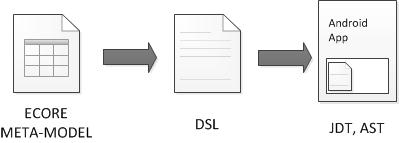
\includegraphics[width=.95\textwidth]{flowchart}
  \caption{Flow chart}
\end{minipage}%
\begin{minipage}{0.5\textwidth}
\label{asttreeview}
  \centering
    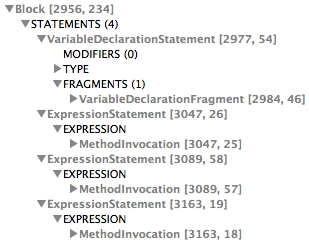
\includegraphics[width=.95\textwidth]{ast}
  \caption{AST of Intent Code}
\end{minipage}%
\end{figure}

We begin by determining the DSL of Android Intents and built our Ecore meta-model which reflected the DSL. Our DSL is based on several examples taken from Open Intents website\footnote{http://www.openintents.org/en/}, the default Android Intents included in Android, and finally the knowledge presented in the chapter \ref{intents}. The final Ecore model is shown the Figure \ref{meta-model}.

\begin{figure}[t]
\label{meta-model}
  \centering
    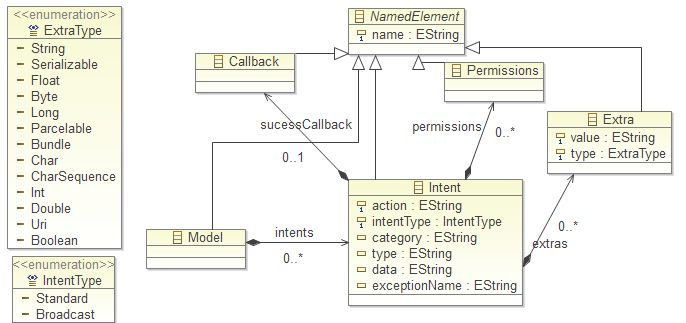
\includegraphics[width=0.9\textwidth]{metamodel}
  \caption{Meta-model of Intent}
\end{figure}

The second stage of development was to take this model and build the Xtext grammar. The final Xtext grammar we produced was based on the default grammar that was generated but with several modifications for simplification and the use of enumerated types. To test the grammar we developed several models based on some examples that we had previously chosen. This allowed us to make changes to both the Xtext grammar and the Ecore model when one or both did not suit the required data from the Intents. The developed models in our DSL are used as our dataset for the plug-in. An example of an Intent in our DSL is shown in the Listing \ref{dsl}.

{\footnotesize\begin{lstlisting}[escapechar=!,label=dsl,caption=Intent in DSL]
ImplicitIntent ActionSendText {
	type "text/plain"
	category "android.intent.category.DEFAULT"
	action "android.intent.action.SEND"
	extras {
		StringExtra "android.intent.extra.TEXT" !$\hookleftarrow$!
		"Put your text here"
	}
},
\end{lstlisting}}

The plug-in uses Model-to-Model transformations, and for this purpose we use JDT and AST as explained in the Section \ref{tools}. The database as defined in our abstract syntax is loaded, and the plug-in interface is built by iterating over the data; the final plug-in interface is presented in the figure \ref{codegeneratorview}. The interface allows a user to choose an Intent and generate the respective code in place where the cursor is. This code is generated through a Model-to-Model transformation from the data held in the abstract syntax to the AST nodes.

The Java code snippet shown in the Listing \ref{loadingDsl}, shows how to load a DSL object into a stand alone Java application with the getBundle() method which allocates specific objects when the application needs to locate such object using this method, it does allow to write independent Java application.

{\footnotesize\begin{lstlisting}[label=loadingDsl,caption=Loading a DSL object into Java application]
public Model getModel() {
	Injector injector = new IntentDslStandaloneSetup().createInjectorAndDoEMFRegistration();
	XtextResourceSet resourceSet = injector.getInstance(XtextResourceSet.class);
	resourceSet.addLoadOption(XtextResource.OPTION_RESOLVE_ALL, Boolean.TRUE);
	Bundle bundle = Platform.getBundle("itu.dk.aamj.intentdsl.ui");
	URL fileURL = bundle.getEntry("gen/i.intentdsl");
	Resource resource = resourceSet.getResource(URI.createURI(fileURL.toString()), true);
	model = (Model) resource.getContents().get(0);
	return model;
}
\end{lstlisting}}

Once the URL which hold the DLS it is a created, we can use the Java annotation Resource, this annotation marks a resource that is needed by the application, these resources responses can Strings or Booleans, in this case the algorithm converts the resource to a string and return it to be use with in the Eclipse Plugin. 
 
The plug-in is capable of handling the three different types of Intent identified; standard Activity Intents, broadcast Intents, and Intents with a callback. The plug-in provides several additional features to aid the developer: searching the dataset, enabling exception handling, producing callback methods if required, and finally the AndroidManifest.xml file is modified with any required permissions. These additional features provide a quick and efficient experience for the developer, with intervention only required when the default settings produced should be modified.

The final plug-in view is shown in Figure \ref{codegeneratorview}. Below we show an example of the generated code for an Intent which sends a customized text to a non specified receiver.

\begin{figure}[t]
\label{codegeneratorview}
  \centering
    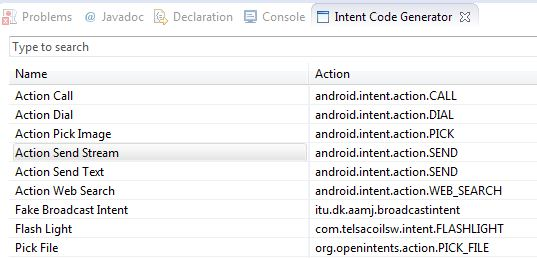
\includegraphics[width=\textwidth]{codegenerator}
  \caption{Final plug-in view}
\end{figure}

{\footnotesize\begin{lstlisting}
Intent ast = new Intent("android.intent.action.SEND");
ast.setType("text/plain");
ast.putExtra("android.intent.extra.TEXT", text);
startActivity(ast);		
\end{lstlisting}}

\section{Evaluation}
\label{evaluation}

\subsection{Method}
\label{Method}
To evaluate our plug-in we will conduct a trial to highlight the benefits of using the code generation that the plug-in provides, as opposed to having developers write the code themselves. Specifically, we aim to show, as stated in the Goals section, that implementation time will be decreased, which encompasses both the coding and correcting of errors. We will base our test primarily on quantifiable data by measuring the difference in time spent creating a group of Intents to be inserted into in a pre-made Android application with just one Activity. The method stubs are left empty for the trial participants to fill out with the correct code, using either the plug-in or by manually writing the code.

The participants were seen as being successful in their trial when they had completed all the required code without errors for the given Intents. The Intents were chosen for their specific use - they were simple, but commonly used. One of the required Intents implementation also required that the developer modify the Android Manifest XML file with a permission required for the Intent to use - for the participants with the plug-in this is handled automatically, but those without had to ensure they correctly inserted it.

The participants, largely made up of students at ITU but with different levels of programming experience, will be split into two groups based on Java programming experience. The least experienced will be instructed to use the plug-in, and the more experienced developers will be asked to do the implementation on their own but are allowed any Internet resource they require. The participants will be given a short introduction to the task first, where they will be given the opportunity to see the fully working application in action on an Android device. After this, the subjects will start the test and the timer started.

It was also considered having participants building the entire application from scratch, but we regressed from this idea because the many variables that this would introduce would make it difficult to dissect the results, and clearly establish the effects of using the plug-in.

\subsection{Results}
\label{Results}
We conducted the trial and recorded the results given in table below:

%Table: http://bit.ly/ZM6rqQ
\begin{center}
\begin{tabular}{|l|l|l|}
    \hline
    ~        & {\bf With the plug-in} & {\bf Without the plug-in} \\ \hline
    ~        & 1:20             & 2:59                \\ \hline
    ~        & 1:08             & 7:02                \\ \hline
    ~        & 1:30             & 4:20                \\ \hline
    ~        & 2:00             & 3:30                \\ \hline
    ~        & 1:09             & 3:20                   \\ \hline
    {\bf Average:} & 1:25             & 4:15                \\ \hline
\end{tabular}
\end{center}

As is palpably shown from the table, the average implementation time was cut severely by a factor of ~3, suggesting that the use of the plug-in may very well contribute to the effectiveness of the developer. These result were very much along the lines of what we had hoped for when we initially set out to create the prototype, and the vast gap in implementation time between the two groups clearly indicates that the use of code generation tools may be of use not only to cut the time spent typing and making documentation lookups, but also to further the correctness of what is written and reduce time spent bug-fixing as a project develops.










\section{Threats to Validity}

\subsection{Internal Validity}
There are several possible problems that can occur when relying on black box testing to ensure the validity of software. The primary concern is ensuring all possible paths through the software have been tested, whether user interaction has avoided possible errors, or simply ignored them, and ensuring all functionality of the software has been tested thoroughly. Some of these possible error situations could be discovered and resolved through automated testing, but by basing our project on existing software with a long history and extensive testing suits, it can be strongly argued for the integrity of our code by ensuring it conforms to all standards.

Our testing method could also be improved upon by including more participants, and increase the amount of testing each participant is required to perform. This would help reduce the amount of potential anomalies in our results, and ensure better test coverage for our plug-in. Our testing would also ideally include experienced Android developers with enough knowledge to be able to write Intent code without the need to look up variables and code structures; this would put a new element into our testing so that we could compare the time taken to write code, against the time taken to open our plug-in, find the correct Intent action, and ensure that the code generated is correctly inserted.

%However, this threat against our plug-in can be extinguished by referring to our original aim, which was to reduce development errors and time taken for developers, by showing that our test results clearly indicate that non-experienced Java developers using our plug-in were significantly faster at developing our test application against experienced Java developers without it.

\subsection{External Validity}

A external validity threat to our plugin is the lack of data that our plug-in holds. Although our dataset covers a wide range of Intents, it is relatively small and therefore we have only tested a very limited set of Intents through our development. It therefore not possible to confirm that our plug-in would work for all of the many Intents available.

In addition to this, without the ability to update the Intent database that our plug-in stores, we cannot ensure that our database has up-to-date and correct information for all Intents available. This could cause potential problems if the Android core Intents were to change in future versions. It is also true that our current dataset cannot guarantee compatibility across all versions of the Android SDK.

\section{Use cases}
\label{usecases}

\label{Use cases}
In the 2011 paper by John Edward Hutchinson titled "An Empirical Assessment of Model Driven Development in Industry", the author brings forth the stories of how a handful of companies in the industry managed to implement an MDD approach to their software development, of particular interest was that of an international Printer Company.
The products of The Printer Company(company names are kept anonymous) are intricate puzzles of mechanical, electrical and software engineering where the embedded software constituted a bottleneck in the development process. The Company slowly introduced MDD on a per project basis with an initial pilot project leading the way for the rest of the product line to undergo same transformation. 
The company's results were astounding in that it led to a reduction in need of man hours but also led to a discovery of greater commonality among their systems, which became the basis for an explicit reuse strategy. After adopting an MDD approach the company was able shorten the time to market and increase the quality assurance.
Similar success stories are reported by other companies in the car industry and telecom industry where the businesses main line of products involve both the mechanical and/or electrical and software engineering disciplines. The use of MDD allows for the programmers to focus on more advanced parts of the development process, while the software base is maintained using an abstract language(DSL) that in and of itself does not require the developer to have an extensive engineering background, but maybe more of a domain expert instead.
This improves the cost-effectiveness and the speed of development, which makes it understandable why companies in the industry are taking an interest to MDD when looking to further their ability to compete in the market.


\section{Related Work}
\label{relatedwork}
While we did go through several papers during the project course these papers are the ones we've considered to be the most relevant.

\textbf{Model2Model Transformation.} In the paper \cite{atl} the authors present ATL (ATLAS Transformation Language) that is a domain-specific language that is designed to solve common Model-to-Model transformation tasks. ATL is a hybrid transformation language, it has declarative and imperative constructs. A module that is a transformation definition in ATL, contains a header section (with a name of the module, source and target models), import sections, helpers (values are specified by OCL expressions) and transformation rules. The authors also present the ATL development tools that are built on top of Eclipse platform which allow developers to perform major tasks, such as compiling, executing, editing and debugging.


\textbf{FSML.} Antkiewicz and Czarnecki wrote an interesting paper concerning FSML \cite{FSML}, where they present the concept of FSMLs with round-trip engineering support. They focus on few challenges related to this topic: knowing how to write framework completion code, viewing the design of the completion code and the migration of the code to the new framework API versions. Framework-Specific Modeling Language (FSML) is a special category of Domain-Specific Language (DSL) that is defined on top of an object-oriented application framework, they model abstractions and rules of application programming interfaces (APIs). FSMLs help developers understand, analyze, create, migrate and evolve application code by showing how applications use APIs. FSMLs are used for expressing framework-specific models of application code, that describe instances of framework-provided concepts that are implemented in the application code. In an FSML each concept instance is characterized by a configuration of features, which represents implementation steps or choices. FSML concept configuration describes how the framework should be completed in order to create the implementation of the concept (how the concept should be implemented in the code). Such models may be connected with the application code through a forward (the generation of code from FSMs by successively executing transformations for code pattern addition), a reverse (the automatic retrieval of FSMs from application code by detecting feature instances in the code) mapping enabling round-trip engineering (RTE). It is possible to implement our plug-in as an FSM, but it would require more effort and time than it is needed since our project is less generic and more specific.


\section{Conclusion}
\label{conclusion}

Our project demonstrates an effective use of Model Driven Development to build systems using multiple layers of abstraction. While the scope of our project may be too small to show its applicability in the industry, the techniques employed have proven to effectively increase the productivity of a software development process when a basis using MDD is established.
With the MDD approach taken during this project process we have addressed the shortcomings of normal high-level languages in respect to excluding platform-specificity and rather introduce domain specific concepts as a means of development. 

As previously mentioned in the Threats to Validity section, the only weak point of our final system is the size of the database used, and that all special cases when working with Intents on the Android platform may not have been fully explored. Automated tests with testing frameworks such as JUnit should also be implemented to ensure correctness over varied scenarios.

The evaluation of the plug-in clearly shows a significant decrease in time taken to develop an error free application when using the plug-in. We can conclude that the plug-in we have created fulfils all of our initial requirements, meets our targeted goals, and also includes some additional functionality that was not set in the base requirements.

\section{Discussion}
\label{Discussion}

Attractive innovation that could be added into the already existing eclipse plug-in are as follows:

- \textbf{Intent dependencies and options.} Adding additional information to the interface such as code previews, descriptions, a list of required permissions, a list of any required dependencies, and possibly links to documentation, would assist the developer during development. Whilst we currently store permissions and callbacks in our database, the additional information would require modifications to the meta-model and DSL. This information would be included alongside the below list in the plug-in interface.

\begin{figure}[H]
\label{codegeneratorview}
  \centering
    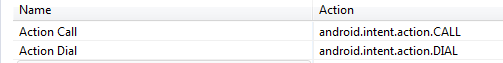
\includegraphics[width=\textwidth]{intentBefore}
  \caption{Future Work 1.0}
\end{figure}

- \textbf{Creating constants and variables}. Many Intents require additional data to perform the call correctly and currently the code generation only inserts pre-defined information as a helper for the developer. A better way of setting this information would be through an interface requesting the user enter the information through the plug-in interface, most probably in a dialog window. This would also resolve the issue that our callback code generation currently has with the variable integer required to detect which call is being returned.

- \textbf{API level support}. Detecting the Android SDK version used, and then modifying the available Intents and code generated for the particular SDK would be a complicated but good feature. This would ensure the code generation works across as many platforms as possible, but compiling the data for each SDK version would be a long and extensive process.

- \textbf{Web-service updates}. Updating the database via a web-service API would ensure the database stays up-to-date and would remove the need to publish new versions of the plug-in when the database should be updated. This would require we setup a server which contains the file but the existing could would remain relatively unchanged, with the only difference being the database file that is loaded.
	

\setlength{\bibsep}{0.0pt}
\bibliographystyle{plain}
\bibliography{references}

\end{document}